\documentclass[10pt]{article}
\usepackage{fullpage,amsthm,amsmath,amssymb,enumitem,url,verbatim,graphicx}
\usepackage{color}
\usepackage{biblatex}
\usepackage{titlesec}
\usepackage{listings}
\usepackage{booktabs}

\addbibresource{references.bib}

\begin{document}

\title{\Large CS 267 Project: Parallelizing Cartesian Tree Construction \\ 
on Multiple Nodes with Partitioned Global Address Space}
\author{\large Andrew Head}
\date{}
\maketitle

% Section resizing hint from
% http://tex.stackexchange.com/questions/103286/how-to-change-section-subsection-font-size
% \titleformat{\section}{\normalfont\fontsize{10}{11}\bfseries}{\thesection}{1em}{}

% \pagenumbering{gobble}

\vspace{-5ex}

\section{Introduction}

This project focuses on adapting an existing parallel algorithm for Cartesian tree construction to
a new parallel architecture: partitioned global address space (PGAS).
We report on a simple but elegant adaptation of the algorithm to PGAS\@.
We describe the key insight---that memory access can be kept mostly local for this
divide-and-conquer algorithm---that motivates our implementation.
Although we fail to outperform the existing technique, we report evidence of sublinear strong and
linear weak scaling for our adaptation, even with multiple nodes (while the original algorithm could run
on only one node).
We describe techniques that we believe may enable performance beyond the baseline algorithm.

\subsection{Motivation}

% The inspiration for this project came from an unlikely source.
The first author's past research focused on automatically generating explanations of
micro-languages like regular expressions~\cite{head_tutorons_2015}.
His aim in this work was to develop a pipeline that would take in arbitrary regular expressions and generate
realistic, readable examples strings of what it matched.

The algorithm we focus on here---Cartesian tree construction, as a first step in suffix tree
construction---was the component of this pipeline where the author found
the most feasible and interesting potential for parallelization using course concepts.
Certain parts of the pipeline, including regular expression matching, are not simple to optimize
beyond ``embarrassingly parallel'' improvements:
Asanovic et al.~\cite{asanovic_view_2009} point out that only `work-inefficient' algorithms are
known for executing finite state machines.
Algorithms have been proposed for improving the speed of regular expression matching through
novel processor architectures (e.g.,~\cite{brodie_scalable_2006}), the use of graphics processing
(e.g.,~\cite{vasiliadis_regular_2009}), splitting input for specific matching
problems~\cite{jones_parallelizing_2009}, and a parallel prefix oriented approach to matching
strings~\cite{hillis_data_1986}.
However, the first author found that, in practice, regular expression matching seemed to be
I/O-bound rather than computation-bound.

While it is not necessarily the bottleneck to the system, an interesting potential resided in
the problem of building a suffix tree at a faster speed.
Initial tests with a 10M file revealed that suffix tree construction with a state-of-the-art
algorithm~\cite{shun_simple_2014} was too slow for interactive automatic explanation speeds---about
two-tenths of a second.
So we set out to improve the speed of this component, particularly because we thought there would
be an interesting problem in refactoring the parallel architecture for the algorithm.
Suffix tree construction is also an active area of research, and it has been for some time.
Suffix trees can provide a fast, often linear-time solution to many string-related problems, 
including finding maximal repeated substrings~\cite{gusfield_algorithms_1997}, making them quite
useful for applications including processing biological sequence
data~\cite{bieganski_generalized_1994}.

\subsection{Related work}

Algorithms for constructing suffix trees have been around for a long time.
Perhaps one of the most-taught algorithms is Ukkonen's, a linear time algorithm for constructing
suffix trees~\cite{ukkonen_online_1995}.
Since Ukkonen, there have been a number of algorithms that have sought to gain even better
performance with the use of parallel tree construction.
The approaches and contexts of each algorithm varies.
I review a set of very recent approaches to provide an overview.
Tsirogiannis et al.\ describe a cache-conscious algorithm tailored to chip-multiprocessor
architectures~\cite{tsirogiannis_suffix_2010}.
Mansour et al.\ develop serial and parallel disk-based suffix tree construction algorithms
optimized to perform well when the string cannot fit completely in main memory~\cite{mansour_era_2011}.
Shun \& Blelloch~\cite{shun_simple_2014} propose the algorithm on which this work is based.
They claim that their algorithm runs in $O\left(\min{d \log n, n}\right)$ time, 
with tree height $d$.
We seek to add a divisor to this runtime, to achieve runtime of
$O\left(\min{\frac{d}{p} \log n, \frac{n}{p}}\right)$.
We are not completely successful in this effort, but we take a first step.

We use their algorithm as a starting point, asking how we can extend their multi-thread single-node
code to run more efficiently on multiple nodes with multiple threads.
In contrast to the other mentioned work~\cite{tsirogiannis_suffix_2010,mansour_era_2011}, we were
not concerned with our input overfilling main memory, and focus on taking advantage of partitioned
global memory rather than memory shared within a multi-processor.

Before proceeding, we take a quick moment to situate this work relative to the \emph{structural}
and \emph{computational} patterns from the CS267 course that relate to this work.
We do not use any of the core computational patterns described by Asanovic et
al.~\cite{asanovic_view_2009}.
While some substring algorithms require a dynamic programming approach, this one uses a fairly
straightforward divide-and-conquer approach (read on for an explanation).
The structural pattern we use (referring not to structure of software, but rather the structure
of memory layout and computation) is \emph{partitioned global address space} (PGAS).
As we were more interested in extending the power of this algorithm by applying a different
structure via another architecture (PGAS) and framework (UPC), we decided to focus our effort in
implementing and evaluating this algorithm under this architecture, rather than exploring
alternative computational patterns for the problem.

\if 0
I discovered that there's a natural extension of a previous algorithm for single-node parallel Cartesian tree construction to multiple nodes using partitioned global address space.
My task was to implement this, and verify whether there were genuine time savings.
\fi

\section{Approach}

Here, we describe our approach to extend the baseline algorithm.
Shun \& Blelloch developed the algorithm with an understanding that a Cartesian tree can be
converted into a suffix tree, when augmented with data from the suffix array it was built from.
A Cartesian tree is a heap produced from an ordered set.
One constraint of its construction is that, when the tree is traversed in order,
it must produce the original ordered
set.\footnote{\url{https://en.wikipedia.org/wiki/Cartesian_tree}}
Shun \& Blelloch showed you could parallelize the construction of a Cartesian tree with a
divide-and-conquer approach.
Cartesian trees are formed from pairs of entries in the ordered set.
These trees are continually merged until you have the Cartesian tree for the set.
Two sub-trees are merged by ordering and linking nodes in the neighboring spines between
two sub-trees.
Shun \& Blelloch implement this with top-down recursion, where the base case merges two nodes, and
a new thread can be spawned for each merge operation on two sub-trees.
We refer the reader to the original paper for details~\cite{shun_simple_2014}.

When considering the most productive way to extend this algorithm to hardware beyond multiple
threads on a single processor, our key insight was as follows:
Given the input as an ordered set, all nodes are merged with their immediate neighbors.
All sub-trees are merged with sub-trees that are neighboring subsets of that ordered set.
The order of the nodes does not change at any time (although individual nodes can be updated with
new links between each of the nodes).
Given that most merge operations would act on only a small chunk of the data (1 merge would
see all of the data, 2 merges would see one-half, 4 would see one-quarter, and so on\ldots{}),
\textbf{exchange of intermediate results between processors simultaneously performing the merge
could be almost completely eliminated by assigning threads and processors a contiguous subset
of the list of nodes and only the computations that performed on those nodes.}
It is not until the last $P - 1$ computations at the last $\log (P)$ levels of the
tree of computation that communication would have to happen at all.
For a graphical representation of this, see Figure~\ref{fig:architecture}.

Our task was then to rewrite the algorithm in a way that:
\begin{itemize}[noitemsep]
  \item Still enabled parallel merging of subtrees
  \item Minimized the communication between distinct ``compute'' nodes
\end{itemize}
The result of our efforts are described in the next two sections.
First, we describe a model that confirms that we should achieve performance improvement by
extending Shun \& Blelloch's algorithm to multiple processors.
Second, we describe how we used a partitioned global address space programming model to support parallel
computation of the Cartesian tree while minimizing communication between nodes.

\subsection{Theoretical Performance}

Prior to doing implementation, we wrote a lightweight model to verify whether utilizing additional
nodes in parallel computation could actually improve performance, given the additional
communication costs it would have to incur in the final merge computations.
Here we walk you through our rationale that confirmed the advantage of using multiple processors.

Define $T_C$ to be a (constant) communication time between processors to transmit a number of
elements that must be used for a merge operation.
Define $T_M$ to be a (constant) merge time for performing a merge computation.
We admit that these quantities are in fact not constant.
But they are likely all within a certain limited range for a tree of a certain depth, and it is
really the ratio between the average communication time and the average merge time that actually
matters when we develop the final cost relation.

For an ordered set of $N$ input elements, there will be in total $N - 1$ merge operations (adjusting
this amount slightly if $N$ is not a power of 2).
If the runtime is defined as purely the amount of time it takes to perform all of the merge
operations, then the runtime on a single processor with one thread will be:
\begin{equation}\label{eqn:single}
T_M * (N-1)
\end{equation}

Consider a second case, where the computation can be shared across multiple processors, but with
a cost of communication every time a merge operation requires elements from another processor.
Assuming the number of elements per processor is a power of 2 and these elements are evenly 
divided across all processors, it is only the final $P - 1$ computations in which processors
must share information (see Figure~\ref{fig:architecture} to verify this with 16 elements
divided between four processors).
The cost of these final computations is now the cost of communication plus the cost of merging,
such that the overall cost of computation with $P$ processors is:
\begin{equation}\label{eqn:multiple}
\left( T_C + T_M \right) *(P-1)+\frac{T_M}{P}*(N-P)<T_M*(N-1)
\end{equation}

As long as Equation~\ref{eqn:multiple} yields a smaller cost than Equation~\ref{eqn:single}, we
reduce cost by using multiple processors.
Simplifying this relationship algebraically, we find that our extensions should achieve speedup
over the single processor baseline as long as the following is true:
\begin{equation}
\frac{T_C}{T_M} < \frac{N}{P} - 1
\end{equation}

In other words, if it takes ten thousand times as long to communicate shared elements between
processors, then there should be about ten thousand times as many elements as there are
processors.
This makes intuitive sense---the longer that communication takes, the more computations will
have to take place with local memory only within each thread to offload the cost of communication.

This cost relationship held with the test data that we used.
With one of our test datasets, we measured an average $T_M$ of 150 ns for each merge.
For their Edison supercomputer, NERSC reports a 250--3700 ns expected communication 
latency.\footnote{\url{http://www.nersc.gov/users/computational-systems/edison/configuration/}}
With 8 compute nodes, we would expect that as few as 200 elements would make parallel merging
with multiple nodes worthwhile.

We also note that although this model was described for the case of single-thread processors,
this relationship extends to the case of multiple threads perfectly sharing work for the single and
multiple-processor cases.
Just add a divisor for the number of threads to the $T_M$ term.

\subsection{Implementation}

\begin{figure}
\centering
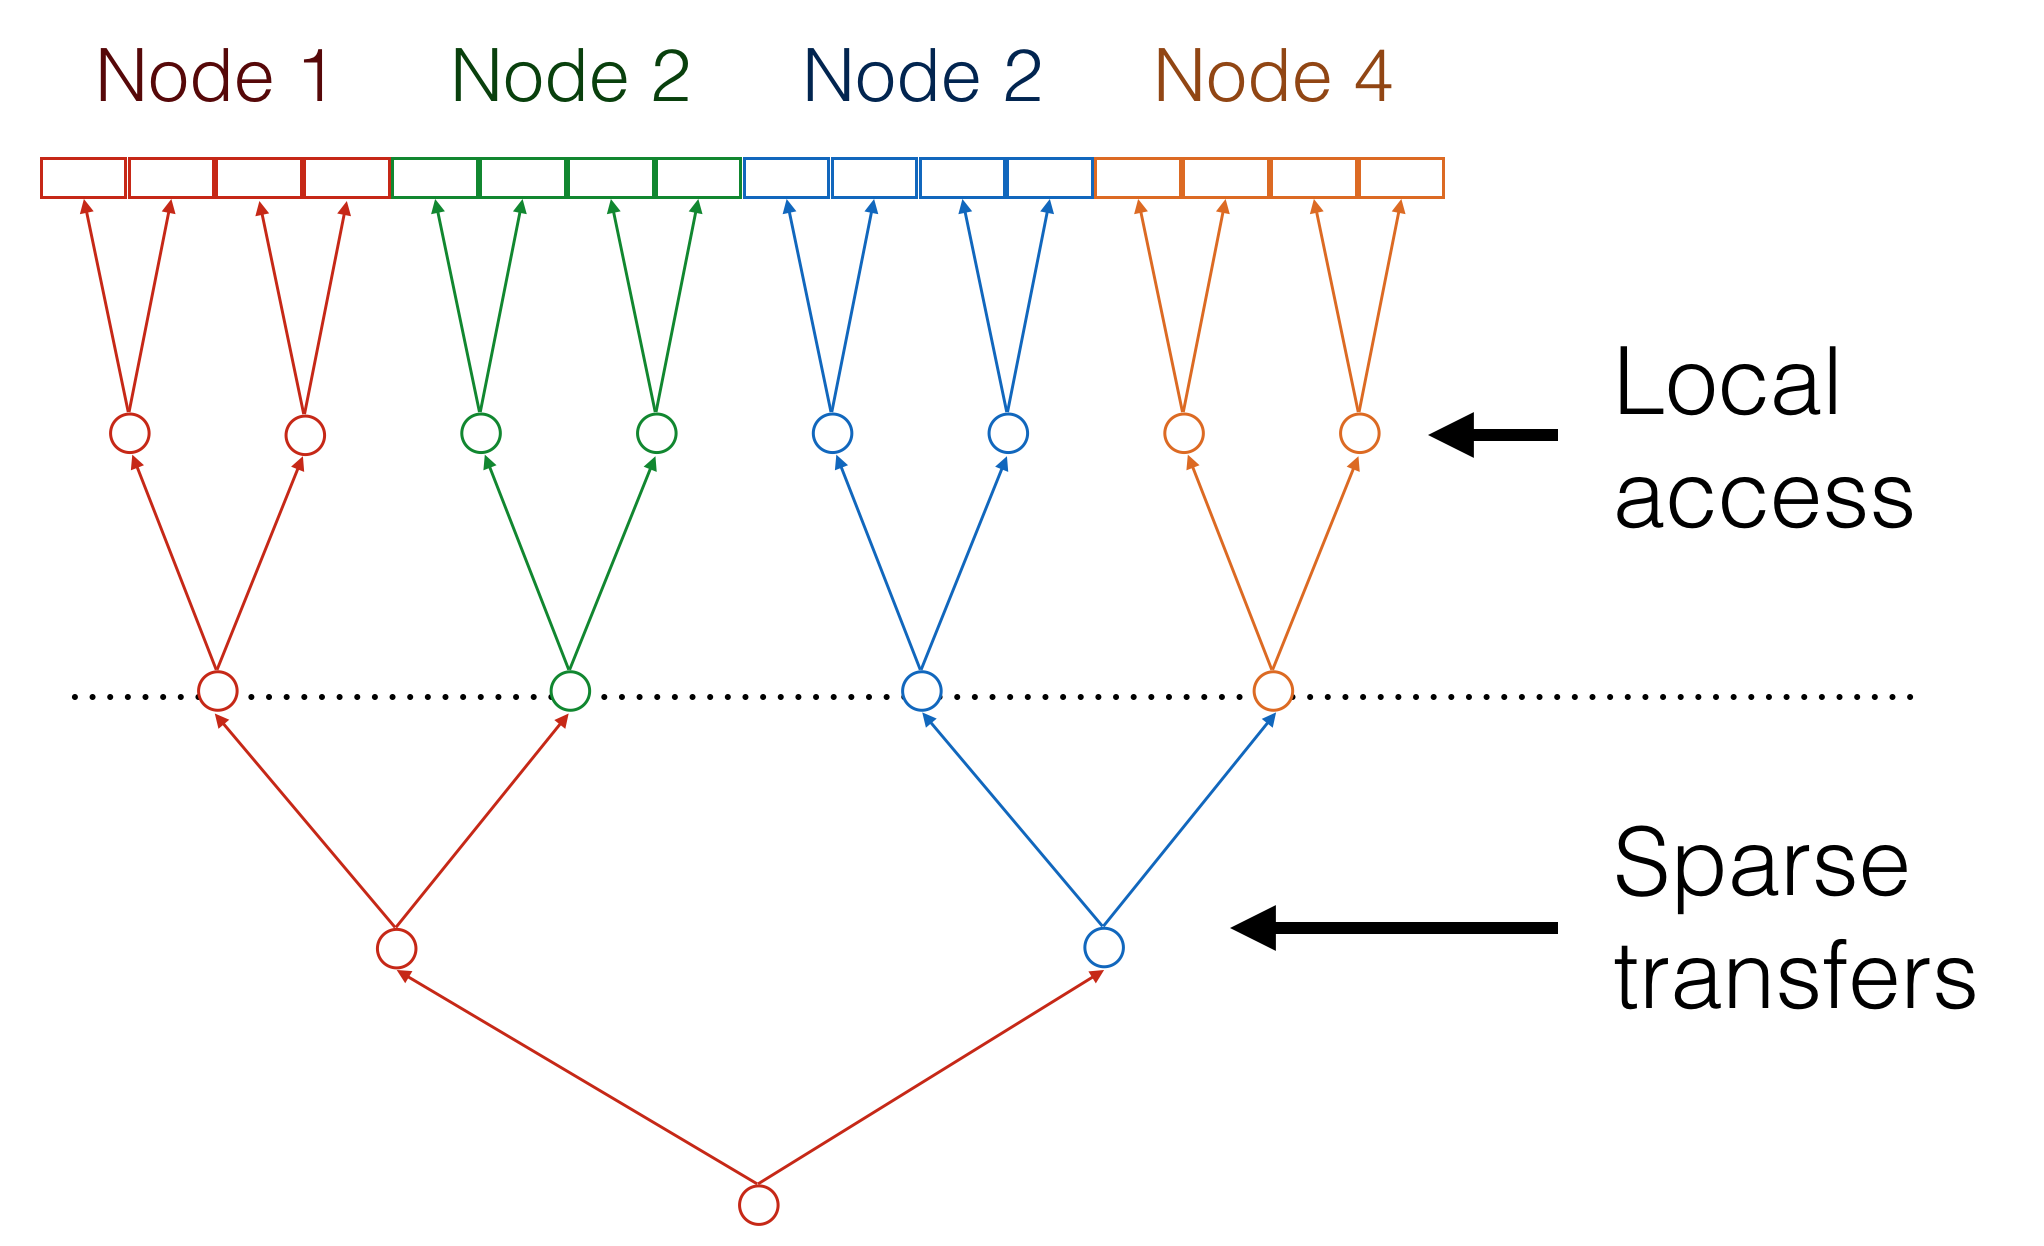
\includegraphics[width=0.6\textwidth]{figures/architecture}
\caption{%
An illustration of what makes partitioned global address space(PGAS) suitable for this algorithm.
The divide-and-conquer algorithm merges the tree by joining contiguous nodes from the ordered set.
As long as we constrain each thread to merge only subtrees in its local memory, all memory accesses will be local until the final $P - 1$ merge operations, where $P$ is the number of processors.
}
\label{fig:architecture}
\end{figure}

Adjusting Shun \& Blelloch's approach of dynamically-spawned threads for divide-and-conquer to
the UPC programming framework required several changes.
Some of these were to support the PGAS programming model;
others were to support syntactic and semantic constraints of the UPC environment.

UPC programs are run with a defined number of threads.
As a result, the number of threads and how memory was divided between them needed to be defined
up front.
We divided the number of entries in the input set evenly between all threads.
Each thread was assigned a contiguous location in the shared list.

We could no longer perform divide-in-conquer in a top-down fashion, as:
\begin{itemize}[noitemsep]
  \item We could no longer spawn new threads at will
  \item Each thread was to only merge its own elements in the common case
\end{itemize}
We refactored the code to perform bottom-up, iterative divide-and-conquer.
In the first iteration, subtrees were merged from pairs of nodes.
In the second, pairs of the subtrees from the first iteration were merged.
Only the UPC thread that `owned' the first node of the left sub-tree performed the merge.
The result was that until the final $P - 1$ computations, all threads accessed only memory with
the affinity to itself.

With a dynamically-sized shared buffer, elements are allocated in round-robin fashion between threads.
Semantically for our algorithm, it was significant that elements that appeared adjacent to each
other in the list were all assigned to the same thread.
To force elements to be inserted into each thread until it was full, we developed a lookup key that
would convert a `cyclic' index of the default round-robin allocation into a block-order index:

\begin{minipage}{\linewidth}
\begin{lstlisting}
for (int i = 0; i < n; i++) {
  thread = i / elements_per_thread;
  phase = i \% elements_per_thread;
  index[i] = thread + phase * THREADS;
}
\end{lstlisting}
\end{minipage}

One disadvantage of this design choice is that it required not one but two index computations
for every array lookup within the shared list.
We discuss this in additional detail in the results section.

The top-down divide-and-conquer approach of the original algorithm implicitly expressed the
dependencies of sub-tree merges:
no merge could be performed until both of the sub-trees it was merging had finished merging
their sub-trees.
As these dependencies were no longer implicitly enforced by bottom-up divide-and-conquer---for
instance, a thread could get far ahead of the others and eventually attempt to merge together its
subtree with an unfinished sub-tree of another thread---we enforced synchronization at each
level of depth within the computation tree using \texttt{upc\_barrier}.

With all of these adjustments, we rewrote the \texttt{cartesianTree} method of Shun \& Blelloch's
code with no more than 23 lines of code (excluding comments and whitespace).
What we want to emphasize here is that this is a simple, elegant iterative solution that allows
the existing algorithm of Shun \& Blelloch to extend to multiple processors, while maintaining
most of the semantics of the original algorithm.
In other words, this program was ripe for adaptation to PGAS.

To demonstrate the elegance of the solution, we show a simplified version of the C code for
our solution here.
Note that the only UPC structures are the share list \texttt{Nodes}, iteration with a level
of the tree using \texttt{upc\_forall}, and synchronization via \texttt{upc\_barrier}.
Some details have been omitted for ease of reading.
For instance, as described above, to access elements by block rather than cyclically, we performed
two array lookups every time we accessed an element of \texttt{Nodes}.

\lstset{language=C}
\begin{minipage}{\linewidth}
\begin{lstlisting}
for (int step = 2; step < n * 2; step *= 2) {
  upc_forall (int start = 0; start < n; start += step; &Nodes[start]) {
    if (n - start >= step) tree_size = step;
    else tree_size = n - start;
    if (tree_size > step / 2) {
      middle = start + (step / 2) - 1;
      merge (Nodes, middle, middle + 1, index);
    }
    upc_barrier;
  }
}
\end{lstlisting}
\end{minipage}

\section{Evaluation}

\subsection{Methodology}

We conducted two tests, for strong and weak scaling, to determine our algorithm's improvement
relative to the Shun \& Blelloch baseline.
For the test of strong scaling, we varied:
\begin{itemize}[noitemsep]
  \item The number of threads on a single processor
  \item The number of processors, with twelve threads per processor
\end{itemize}
to determine whether our algorithm scaled with the amount of computational power afforded to it.
We performed Cartesian tree construction on a set of 20,971,521 elements, representing the suffix
tree for a text 10\texttt{M} in size.
This was an excerpt of the file
\texttt{etext-99}.\footnote{\url{http://people.unipmn.it/manzini/lightweight/corpus/etext99.bz2}}

We also conducted a test to assess weak scaling.
We observed the performance of our code on suffix arrays built from text files of size 
500\texttt{KB}, 1\texttt{MB}, 2\texttt{MB}, and 4\texttt{MB}.
Each of these text files was formed from the head of the \texttt{etext-99} file.
The tests therefore had to operate on about 1, 2, 4, and 8 million elements each.
All tests were run on two processors with twelve threads each.

\subsection{Results}

\begin{figure}[t]
\centering
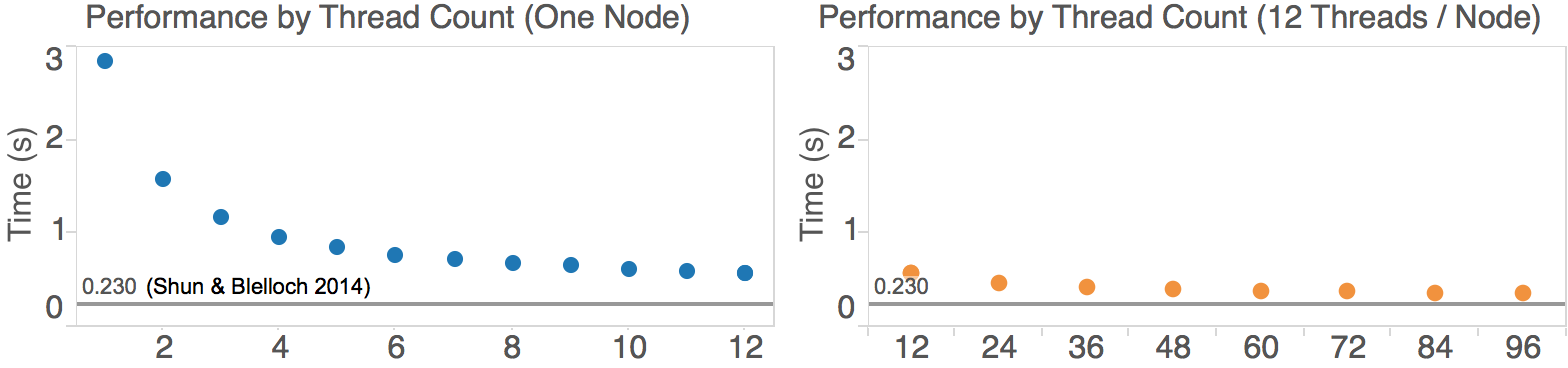
\includegraphics[width=0.8\textwidth]{figures/benchmarks}
\caption{%
Results of benchmarks on our algorithm.
There are three groups of plots in this figure, from top to bottom.
The first pair plots the runtime of our algorithm against the number of threads.
The blue plot represents a single processor with up to twelve threads;
the orange plot represents multiple processors, each with twelve threads.
The ``Shun \& Blelloch 2014'' reference line reports the performance of the algorithm on which
this one was based, which used a dynamic number of threads on a single processor.
The second pair of plots shows these same runtimes on a log-log scale.
This shows evidence of strong scaling, albeit sub-linear.
The final plot with green points shows the weak scaling of this algorithm, reporting how
performance of the algorithm changes as you increase the number of input elements.
}
\label{fig:benchmarks}
\end{figure}

After benchmarking performance with these measures on the NERSC Edison machine,
we observed the following.
As we increase the number of threads and processors, we see evidence of strong scaling.
That is, increasing the computational resources decreases the amount of time computation takes.
However, this is sublinear.
The log-log plots in the second row of Figure~\ref{fig:benchmarks} curves slightly beneath what
would be a straight line from the first point to the last point.
Our algorithm also achieves weak scaling with multiple processors.
We see a linear relationship between the size of the input and the amount of time that our
Cartesian tree algorithm takes.
The results of our two tests are summarized in the plots of Figure~\ref{fig:benchmarks}.

We take care to note that, somewhat unexpectedly, \emph{none} of our configurations perform better
than the Shun \& Blelloch source code on which our approach was based, not even the configurations
that make use of multiple processors (see the reference line in Figure~\ref{fig:benchmarks}).
We describe in the next section why we think this is.
In short, we attribute the poor performance to overhead from UPC together with strict 
synchronization.
Despite this, we still see ourselves as achieving part of our goal of observing strong scaling with
our algorithm with multiple nodes beyond its performance on a single node.

\subsection{Diagnostics}

We did not expect our adjustments to the algorithm to add such overhead that we could not
improve on the baseline performance of Shun \& Blelloch even with 8 simultaneous nodes.
The time increase occurred in the execution of the algorithm itself, ignoring the cost of loading
input and writing out results for our benchmark.
We observed that our algorithm took double the time that in the merge operation, and six times
as long in the Cartesian tree construction algorithm that invokes merges
(see Table~\ref{tab:method_performance}).

\begin{table*}[t]
\caption{Runtime of methods before and after our modifications}
\vspace{1.5ex}
\label{tab:method_performance}
\centering
\begin{tabular}{lll}
\toprule
\textbf{Method} & \textbf{Implementation} & \textbf{Time} \\
\midrule
\texttt{merge} & ours & 0.45s \\
\midrule
\texttt{cartesianTree} & ours & 0.24s \\
\midrule
\texttt{merge} & Shun \& Blelloch 2014 & 0.22s \\
\midrule
\texttt{cartesianTree} & Shun \& Blelloch 2014 & 0.04s \\
\bottomrule
\end{tabular}
\end{table*}

To determine what caused this overhead, we took effort to profile the code in two ways.
First, we profiled our code with the \texttt{gprof} utility according to the instructions from
the UPC user guide.\footnote{\url{http://upc.lbl.gov/docs/user/#profiling}}
Second, we analyzed our program's UPC memory access and synchronization using 
\texttt{upc\_trace}.\footnote{\url{http://upc.lbl.gov/docs/user/#tracing}}
We describe key performance measurements in Table~\ref{tab:trace_measurements}.
We note that profiling and tracing both add overhead that may make the relative time spent on
operations that we measure unrepresentative of uninstrumented execution.

\begin{table*}[t]
\caption{Runtime statistics generated by \texttt{upc\_trace}}
\vspace{1.5ex}
\label{tab:trace_measurements}
\centering
\begin{tabular}{ll}
\toprule
\textbf{Measure} & \textbf{Value} \\
\midrule
Runtime (per thread) & 70.22s \\ \midrule
Runtime (total, all threads) & 842.64s \\ \midrule
Time waiting in \texttt{upc\_barrier} & 90.6s \\ \midrule
UPC 'get' operations & 1,363,142 \\ \midrule
UPC 'put' operations & 1,363,145 \\ \bottomrule
\end{tabular}
\end{table*}

With these measurements, I expect these factors contributed to the overhead of our
implementation:
\begin{itemize}
  \item \emph{Thread count}.
        On NERSC's Edison machine, each compute node has 12 cores with 1-2 
        threads.\footnote{\url{http://www.nersc.gov/users/computational-systems/edison/configuration/}}
        We assumed that performance would degrade after 12 threads per node, so we didn't
        bother testing more than this count.
        As the Shun \& Blelloch algorithm placed no explicit upper limit on the number of threads
        that could be running at any time, it's possible that more threads were running, resulting
        in a higher CPU utilization.
  \item \emph{\texttt{upc\_barrier}}.
        Of the 842.64 seconds spent by all threads during the UPC trace, 90.6 seconds was
        spent waiting at a \texttt{upc\_barrier}.
        This is only one-tenth of the total runtime of the trace.
        However, if much more time is spent at the barrier in code that has not been instrumented
        for tracing, relative to the total runtime, this could cause threads to waste time
        synchronizing with each other that wasn't present in the Shun \& Blelloch algorithm.
  \item \emph{Costly shared memory access}.
        Access to individual elements in the input ordered set is slowed down by two modifications
        in our implementation.
        First, each index had to be converted from block-based addressing to cyclic addressing.
        Second, the cyclic addressing had to be converted from an address to shared memory to a
        physical memory location.
\end{itemize}

Appropriate adjustments addressing each of these observations include, in increasing order of
difficulty:
\begin{itemize}
  \item Increase the number of threads per node.  This is the simplest adjustment, as it would
        require only to change the arguments passed to the \texttt{upcrun} command.
  \item Cast pointers to shared data types to pointers to private data for all merge operations
        until a thread needs to access nodes shared in other threads' memories.
        This reduces the cost of converting shared memory addresses into a private address with every
        access.
  \item Use an equally conservative but less costly synchronization method.
        For example, UPC locks on heads of sub-trees could be used instead of barriers.
        In such an implementation, each thread would have to wait only for its neighboring threads
        to complete merging their sub-trees, instead of waiting on all other threads to finish
        their computations at each level of the computation tree.
  \item Extend the UPC source code to support block-based indexing instead of cyclic indexing.
        This would eliminate the need to convert the index in each iteration from a cyclic index
        into a block-order index.
\end{itemize}

With the array of existing profiling tools for UPC, we found it difficult to measure
the time computing shared array indexes and waiting at barriers.
With the low cost of the first two adjustments, these two are
certainly worth implementing in near future iterations of this algorithm.
A deeper understanding of the time spent at barriers and computing indexes is needed before we
could justify the cost of implementing them.
With these improvements, I expect that our PGAS extension of the Shun \& Blelloch algorithm can
achieve both superior performance and strong scaling when run on multiple processors.

\section{Conclusion}

We proposed an extension to a parallel Cartesian tree construction algorithm that enables it to
scale across multiple processors using partitioned global address space.
We presented a model that suggests that performance improvement should be seen with multiple processors 
for all but non-trivial input sizes.
We demonstrated that an implementation of our algorithm achieves sub-linear strong scaling with
the number of processors used, and that the algorithm also shows weak scaling.
After finding that our algorithm does not yet surpass the performance of the algorithm on which
it is based, we proposed adjustments to compensate for the additional costs of implementing
it using an architecture within the UPC framework.

Thank you to the course instructors for introducing the first author to the tools and concepts
needed to consider improving the parallel code in the domain of string analysis.
Thank you especially to Marquita Ellis for a constructive conversation to clarify
this project's aims, and Orianna DeMasi for her suggestions on how to improve the post-mortem
for our algorithm and performance reporting.

\printbibliography{}

\end{document}
